\tikzset{
  sioarrow/.style={-{Latex[length=2.7mm,width=1.8mm]},line width=.8pt,draw=black!75},
  sioforward/.style={-{Latex[length=2.7mm,width=1.8mm]},line width=1pt,draw=SIOBlue},
  sioreturn/.style={-{Latex[length=2.7mm,width=1.8mm]},line width=1pt,draw=SIOGreen},
  sionodeblue/.style={rounded corners=3pt,draw=SIOBlue,line width=.8pt,fill=SIOBlueLight,align=center,inner sep=7pt},
  sionodegreen/.style={rounded corners=3pt,draw=SIOGreen,line width=.8pt,fill=SIOGreenLight,align=center,inner sep=7pt},
  sionodeneutral/.style={rounded corners=3pt,draw=SIOGray,line width=.7pt,fill=SIOGrayLight,align=center,inner sep=7pt},
  sionodeochre/.style={rounded corners=3pt,draw=SIOOchre,line width=.8pt,fill=SIOOchreLight,align=center,inner sep=7pt}
}

\newcommand{\SIOFigureOne}{%
\begin{figure}[htbp]
\centering
\begin{tikzpicture}[font=\small,node distance=18mm and 34mm]
  \node[sionodeblue,text width=42mm] (S) {\textbf{Absolute Subjectivity}\\[2pt]$S$};
  \node[sionodeneutral,text width=42mm,right=of S] (R) {\textbf{Relative Subjectivity}\\[2pt]$R$};
  \draw[sioforward] (S) -- node[above,fill=white,inner sep=2pt]{Projection} (R);
  \coordinate (M) at ($(S)!0.5!(R)+(0,-19mm)$);
  \node[sionodeneutral,text width=42mm,inner sep=4pt] (I) at (M) {\textbf{Constitutive intersection}};
  \node[sionodegreen,text width=52mm,below=18mm of I] (X) {\textbf{Intersection Subjectivity}\\[2pt]$X$};
  \draw[draw=SIOGray,line width=.7pt] (S.south) -- (I.north west);
  \draw[draw=SIOGray,line width=.7pt] (R.south) -- (I.north east);
  \draw[sioarrow] (I) -- (X);
  \node[draw=SIOGray,rounded corners=6pt,fit=(S)(R)(I)(X),inner sep=7mm,label={[text=SIOGray]above:Triadic ontological self-closure}] {};
\end{tikzpicture}
\caption{Ontological prototype of Subjectivity Intersection Ontology. Relative Subjectivity $R$ is differentiated through the projection of Absolute Subjectivity $S$, and Intersection Subjectivity $X$ emerges through the constitutive intersection of $S$ and $R$. The diagram represents a triadic ontological closure, not a temporal sequence or an empirical mechanism.}
\label{fig:ontological-prototype}
\end{figure}%
}

\newcommand{\SIOFigureTwo}{%
\begin{figure}[htbp]
\centering
\begin{tikzpicture}[font=\small,node distance=30mm and 46mm]
  \node[sionodeblue,text width=38mm] (A) {\textbf{Relative Subjectivity}\\[2pt]$A$};
  \node[sionodeblue,text width=38mm,right=of A] (B) {\textbf{Relative Subjectivity}\\[2pt]$B$};
  \node[sionodegreen,text width=48mm,below=31mm of $(A)!0.5!(B)$] (C) {\textbf{Intersection Subjectivity}\\[2pt]$C$};
  \draw[sioforward] (A.south east) -- (C.north west);
  \draw[sioforward] (B.south west) -- (C.north east);
  \node[fill=white,inner sep=2pt,text=SIOBlue] at ($(A)!0.5!(B)+(0,-18mm)$) {Constitutive intersection};
  \draw[sioreturn] (C.west) to[bend left=42] node[below left,text=SIOGreen]{reconstitution of $A$} (A.south);
  \draw[sioreturn] (C.east) to[bend right=42] node[below right,text=SIOGreen]{reconstitution of $B$} (B.south);
  \node[draw=SIOGray,rounded corners=6pt,fit=(A)(B)(C),inner sep=8mm,label={[text=SIOGray]above:Canonical operational closure}] {};
\end{tikzpicture}
\par\smallskip
\fcolorbox{SIOGray}{SIOGrayLight}{\strut\textbf{Arrows denote constitutive dependence rather than temporal sequence.}}
\caption{Canonical operational closure among multiple Relative Subjectivities. Relative Subjectivities $A$ and $B$ constitute Intersection Subjectivity $C$ through perspective intersection; $C$ in turn reconstitutes $A$ and $B$.}
\label{fig:operational-closure}
\end{figure}%
}

\newcommand{\SIOFigureThree}{%
\begin{figure}[htbp]
\centering
\resizebox{.96\textwidth}{!}{%
\begin{tikzpicture}[font=\small]
  \foreach \x/\n/\a/\b in {
    0/N1/Third-subject status/and irreducibility,
    3.2/N2/Generation through/intersection,
    6.4/N3/Reconstitution of/originating subjectivities,
    9.6/N4/Ontological status/of the candidate third,
    12.8/N5/General theoretical/scope}{
      \node[sionodeblue,text width=29mm] (\n) at (\x,0) {\textbf{\n}\\[2pt]\a\\\b};
  }
  \node[sionodeneutral,text width=58mm] (J) at (6.4,-2.2) {\textbf{Logical conjunction}\\[2pt]\textbf{(N1--N5)}};
  \node[sionodegreen,text width=57mm] (N6) at (6.4,-4.1) {\textbf{N6}\\[2pt]Integration of N1--N5 within one ontology};
  \foreach \n in {N1,N2,N3,N4,N5}{\draw[draw=SIOGray,line width=.7pt] (\n.south) |- (J.north);}
  \draw[sioarrow] (J) -- (N6);
\end{tikzpicture}}
\par\smallskip
\textit{N6 is a conjunction condition---not an additional or additive score.}
\caption{Logical relation among the comparative criteria. N1--N5 are independent, non-additive structural criteria. N6 is their conjunction condition.}
\label{fig:criteria-conjunction}
\end{figure}%
}

\newcommand{\SIOFigureFour}{%
\begin{figure}[htbp]
\centering
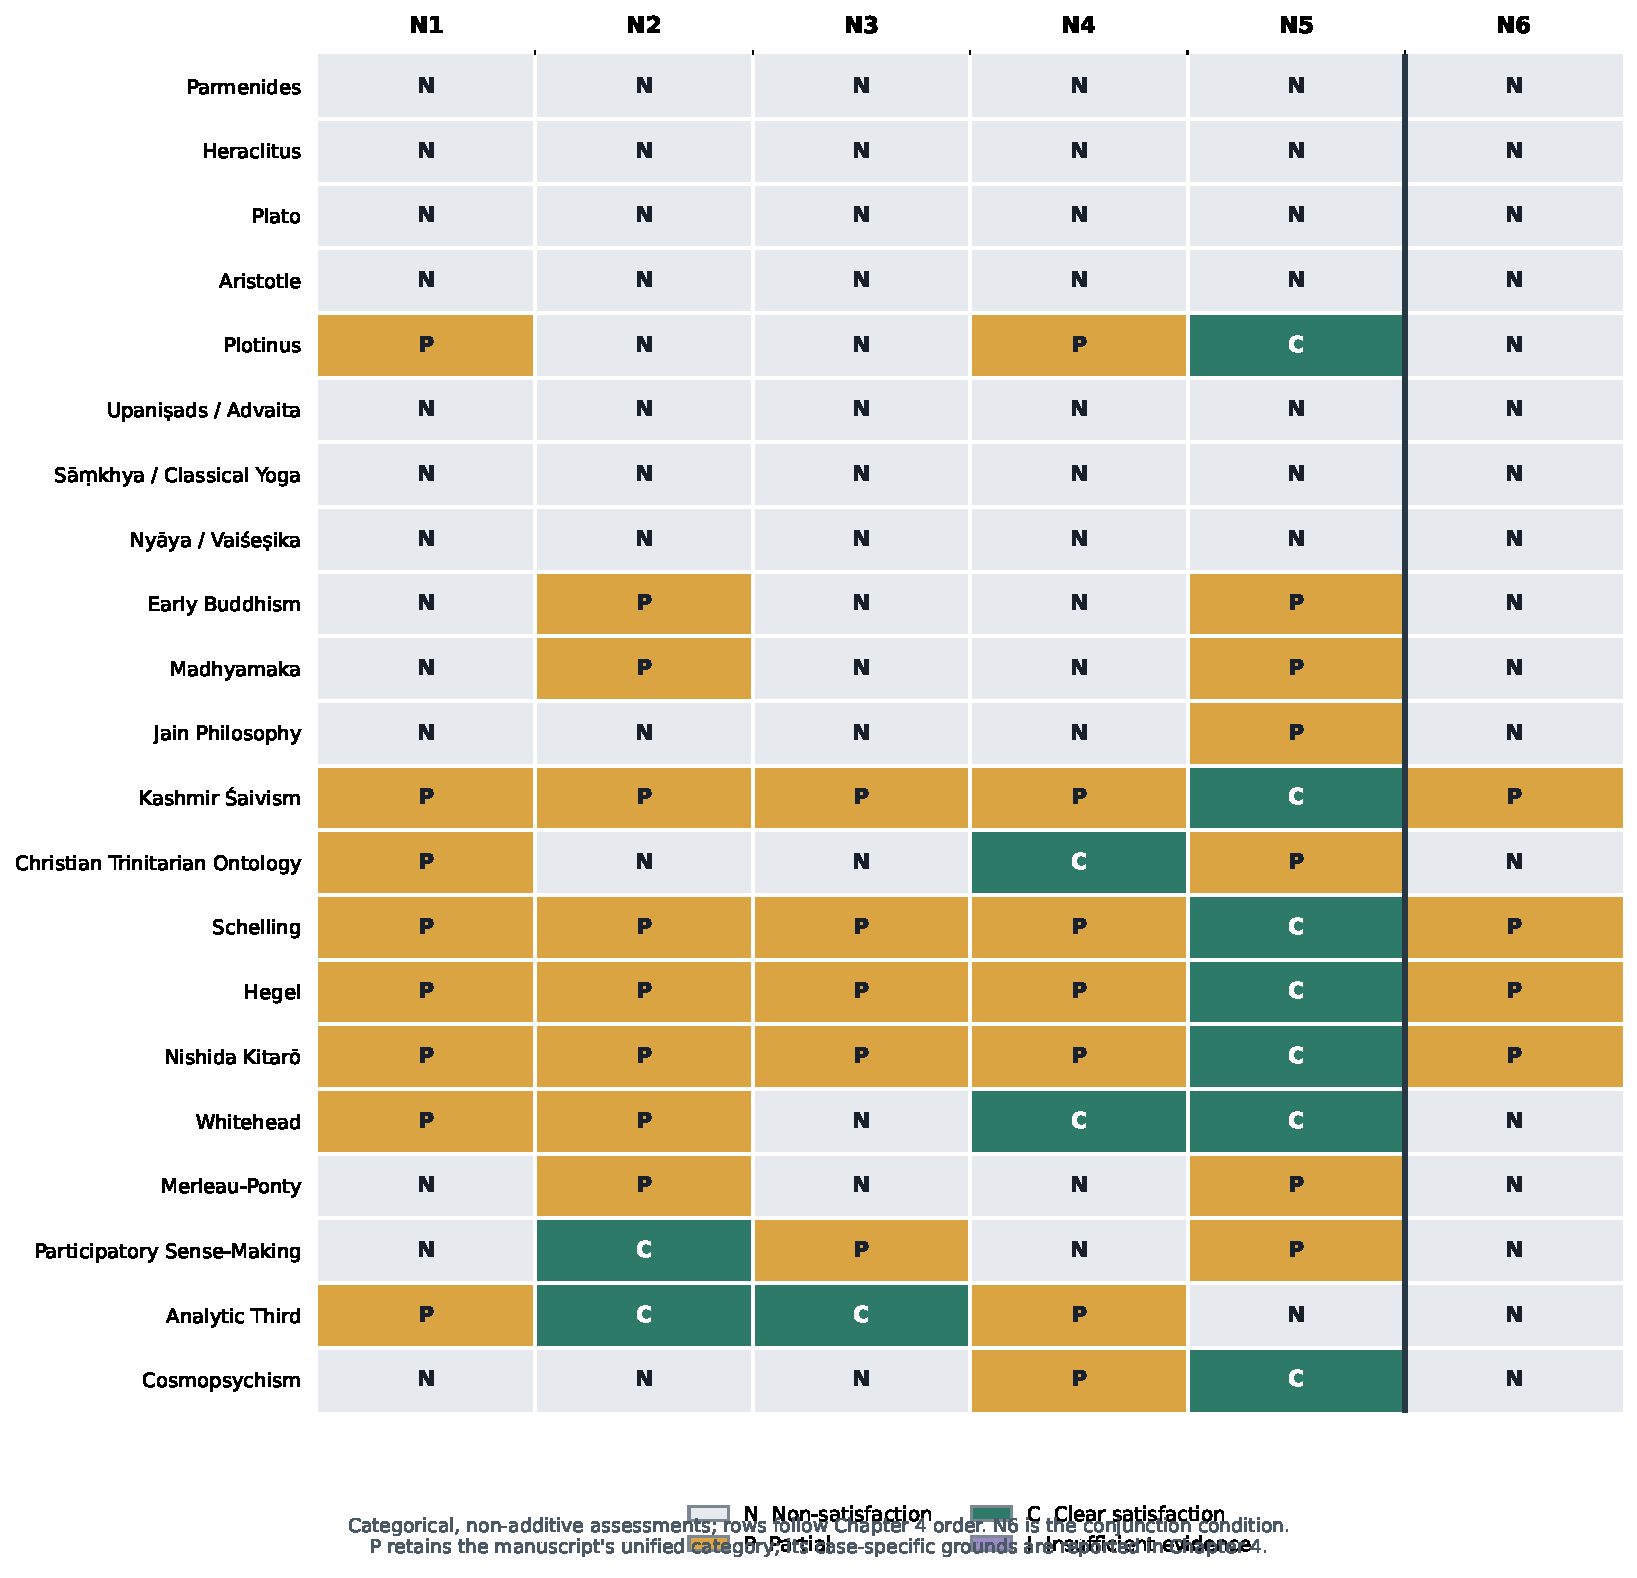
\includegraphics[width=.96\textwidth]{../../figures/output/figure-4-comparative-matrix.pdf}
\par\smallskip
{\scriptsize
\colorbox{MatrixN}{\strut\textbf{N}} = non-satisfaction\quad
\colorbox{MatrixP}{\strut\textbf{P}} = partial or interpretation-dependent\quad
\colorbox{MatrixC}{\strut\textcolor{white}{\textbf{C}}} = clear satisfaction\quad
\colorbox{MatrixI}{\strut\textbf{I}} = insufficient evidence\par}
\caption{Distribution of criterion-level assessments across the comparison set. Rows follow the order of the historical review. The categories are non-additive and do not rank the philosophical value or historical importance of the comparison cases. N6 is separated visually because it assesses the conjunction of N1--N5. P retains the single category defined in Chapter 3; its case-specific grounds are reported separately in Chapter 4.}
\label{fig:comparative-matrix}
\end{figure}%
}

\newcommand{\SIOFigureFive}{%
\begin{figure}[htbp]
\centering
\resizebox{.94\textwidth}{!}{%
\begin{tikzpicture}[font=\scriptsize,node distance=5mm]
  \node[sionodeblue,text width=21mm,minimum height=17mm,inner sep=4pt] (O) {\textbf{Ontological definition}\\[2pt]What is proposed?};
  \node[sionodeneutral,text width=21mm,minimum height=17mm,inner sep=4pt,right=of O] (F) {\textbf{Formal hypotheses}\\[2pt]How represented?};
  \node[sionodeneutral,text width=21mm,minimum height=17mm,inner sep=4pt,right=of F] (P) {\resizebox{20mm}{!}{\textbf{Operationalization}}\\[2pt]What is observable?};
  \node[sionodegreen,text width=21mm,minimum height=17mm,inner sep=4pt,right=of P] (E) {\textbf{Empirical testing}\\[2pt]Discriminate alternatives?};
  \node[sionodeochre,text width=21mm,minimum height=17mm,inner sep=4pt,right=of E] (R) {\textbf{Revision or rejection}\\[2pt]What changes or fails?};
  \draw[sioarrow] (O) -- (F);
  \draw[sioarrow] (F) -- (P);
  \draw[sioarrow] (P) -- (E);
  \draw[sioarrow] (E) -- (R);
  \coordinate (FlowMid) at ($(O.south)!0.5!(R.south)$);
  \draw[sioreturn] (R.south) -- ++(0,-1.55) -| (O.south);
  \node[text=SIOGreen,align=center,fill=white,inner sep=2pt] at ($(FlowMid)+(0,-15.5mm)$) {feedback to ontological assumptions, formal models,\\and operational definitions};
\end{tikzpicture}}
\par\smallskip
\textit{No formalization, operationalization, or empirical result, by itself, validates the ontological proposal.}
\caption{SIO as a formal and empirical research program. Ontological definition, formalization, operationalization, and empirical testing remain distinct stages. Empirical results may require revision or rejection of an operational hypothesis, formal model, or ontological assumption.}
\label{fig:research-program}
\end{figure}%
}
